\section{Real-time Ethernet networks}\label{sec:rt-networks}

% What are they
As explained in \autoref{sec:context}, real-time \emph{Ethernet} networks have strict timing requirements which makes the usage of common \emph{Ethernet} not adequate.
The IEEE 802.3 standard, as is, does not guarantee a deterministic timing for the delivery of message packets.
As such, a few adaptations of this standard have surfaced over the years, focusing mostly on providing this deterministic delivery of, at least, the message packets that are critical for the system.

% General Characteristics
Commercial \emph{Ethernet} is based upon a 7-layer addressing scheme named \textbf{OSI} (\textbf Open \textbf Systems \textbf Interconnection).
Adaptations such as \emph{Ethernet/IP} or \emph{Profinet/IO} still make use of this 7-layer scheme but manage on which layer message packets are sent, depending on their priority.
On the other hand, implementations such as \emph{EtherCAT} drop most of the \emph{OSI} model and create an entirely new addressing scheme based on the model's second layer.

\subsection{EtherCAT} \label{sec:ethercat}

\subsubsection{Working principle} \label{subsec:ecat_principle}

The \emph{EtherCAT} protocol employs a master/slave configuration where only the former is allowed to initiate a data transfer.
Effectively this means the master node is responsible for maintaining periodic communication with all nodes.
The master device requires a simple \emph{Ethernet} \textbf Medium \textbf Access \textbf Controller ({\bfseries MAC}), meaning it can be implemented in virtually any device with a standard \emph{Ethernet} port, and programmed with any real-time operating system and software.
Slave devices require an \textbf \emph{EtherCAT} \textbf Slave \textbf Controller ({\bfseries ESC}) which processes the frames entirely in hardware.
This allows the network performance to be predictable and independent of specific slave device implementations.

The \emph{EtherCAT} frame sent by the master passes through each and every node on the network until it is sent back to it by the last node in each branch.
Because slave devices use a specialized communication chip, their data is inserted in the frame ``on the fly''.
This means that the master node can exchange data with every node on the network with a single \emph{EtherCAT} frame.


\subsection{The protocol} \label{subsec:ecat-protocol}

The \emph{EtherCAT} protocol embeds its own frames into a standard \emph{Ethernet} frame, signing it with an hexadecimal value of $\mathtt{0x88A4}$ on the \emph{Ethernet}'s type header field.
Other protocol stacks like TCP/IP or UDP/IP can be used concurrently with \emph{EtherCAT}, but they are not required.
These are encapsulated into a separate mailbox so they do not disrupt real-time process data transmissions.
The fact that this network does not use these stacks means it has lower communication overhead.

The \emph{EtherCAT} frames are, themselves, divided into several datagrams, as show in \autoref{fig:ecat-frame}.
These can be addressed to specific devices using their node address or be sent to multiple devices, concurrently, using a logical address.
The datagram header contains information about the type of operation to perform, which can be one of three options: read, write of concurrent read-write operations.

\begin{figure}[htp]
	\centering
	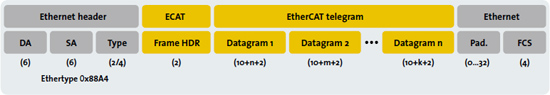
\includegraphics[width=0.8\textwidth]{EtherCAT_Technology_01_Protocol.jpg}
	\caption{EtherCAT frame structure \cite{protocol:ethercat}}
	\label{fig:ecat-frame}
\end{figure}

Datagrams include all information regarding data access which permit the master device to decide what data to access and when, meaning a fixed process data structure is not required.
Effectively, master devices can update variables with different cycle times, possibly relieving some processing power.
As an example, for a system that requires motion control, the motor drives can get their parameters updated with a 1ms period, while discrete Inputs/Outputs (I/Os) can be updated with a 20ms period (typical control applications).

Each slave contains a unique node address which is assigned during network configuration.
Because node addresses are static, they can be used to target the specific node, even if the underlying network topology changes.
In addition, slaves can also be addressed by their location on the network, but this is usually only used during network initialisation to check for topology changes.
This is done by comparing a configured list of node addresses and their location on the network with the discovered topology.

On system initialisation, multiple logical addresses can be configured on each node, allowing a single datagram to target multiple physical devices.
The cyclical exchange of process information uses logical addressing to execute the data transfers.

This type of addressing scheme also allows slave-to-slave communication.
There are two possibilities of achieving this:
\begin{enumerate}
	\item If the process structure is constant, sending data to another slave which is further downstream can be done in the same bus cycle;
	\item If the process is not constant or the network has a dynamic topology, slave-to-slave communication can go through the master device and, because of \emph{EtherCAT}'s performance, this is still faster than other traditional communication stacks (TCP/IP, UDP/IP, etc.).
\end{enumerate}

EtherCAT can also benefit from the modern system's \textbf Direct \textbf Memory \textbf Access (DMA) feature, which removes the necessity for a CPU to explicitly transfer data from physical RAM to a peripheral device.
This means that a master device application only needs to construct the EtherCAT frame and place it on a specific memory region, leaving the DMA controller to actually pass the data over to the Ethernet MAC controller, saving CPU for the actual data processing.


\subsubsection{Topology}

\emph{EtherCAT} supports a variety of network topologies like \emph{line}, \emph{tree}, \emph{star} or \emph{daisy-chain}.
When designing a certain network, multiple topologies can be combined into a hybrid topology network.
Many ESCs and Input/Output (I/O) modules already include ports to create network branches, which eliminates the need to use switches or any other type of infrastructure components.
Regardless, classical \emph{Ethernet} star topology can be used to implement an \emph{EtherCAT} network.

ESCs also include support for a ``Hot Connect'' feature which means existing nodes can be removed and new nodes can be added to the network during runtime.
The controllers can detect these changes in a very short time (typically less than 15$\mu$s), allowing a smooth state transition without interfering with the rest of the network.

There is also a big flexibility in terms of available cabling option, from inexpensive industrial \emph{Ethernet} cables to fiber optics, having the entire Ethernet wiring possibilities available for use.

EtherCAT gateways provide the means to incorporate other fieldbus networks as a subnetwork.
This allows a gradual changeover between fieldbuses by keeping network sections that may contain components which still do not support the EtherCAT interface.

Due to the fact that EtherCAT uses a 16-bit address length, up to $65535$ devices can exists in a single network segment, which makes scalability virtually unlimited.
This large device count removes the need to use bus extension methods, like traditional gateways, providing even the largest EtherCAT networks the best possible performance without delays.



\subsection{Ethernet/IP} \label{sec:ethernetip}




\subsection{Profinet/IO} \label{sec:profinetio}



